 \providecommand{\main}{../../..}
\documentclass[\main/main.tex]{subfiles}
\begin{document}
\subsection{Esercizio 1}
Dato il seguente problema di PL:

\begin{figure}
  \begin{align*}
    \min z = -2x_1 + x_2    \\
    -3x_1 + 10x_2 & \geq 0  \\
    x_1 + x_2     & \leq 13 \\
    x_2           & \leq 5  \\
    -x_1 + x_2    & \leq 3  \\
    x_1, x_2      & \geq 0
  \end{align*}
  \caption{Esercizio 1}
\end{figure}

\begin{enumerate}
  \item Si disegni la regione ammissibile e si evidenzi il vertice ottimo per via grafica, riportando il valore di z e di tutte le variabili del modello, comprese quelle di scarto.
  \item Si risolva mediante gli scarti complementari il duale del problema.
\end{enumerate}

\subsection{Soluzione esercizio 1}

\subsubsection*{Identifico soluzione ottima}

\begin{figure}
  \begin{subfigure}{0.49\textwidth}
    \dddgraph{x_1}{x_2}{0}{10}{0}{5}{-10}{
      -3*x + 10*y >= 0&&
      x + y <= 13 &&
      y <= 5 &&
      -x+y<=3
    }{-2*x+y}
    \caption{Il vertice ottimo ha coordinate $\bmx = \rnd{10,3}$}
  \end{subfigure}
  \begin{subfigure}{0.49\textwidth}
    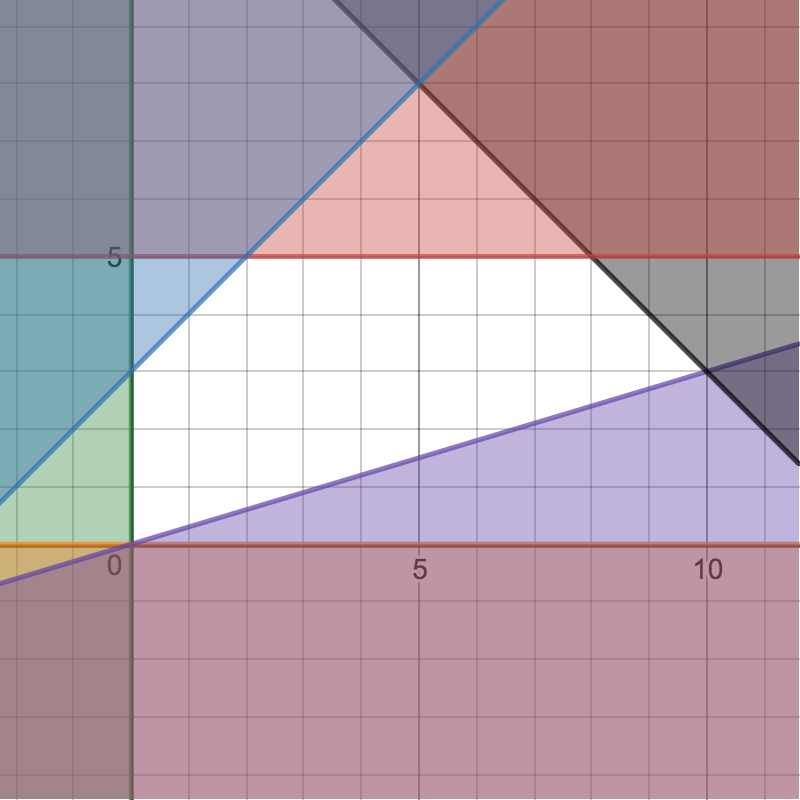
\includegraphics[width=0.9\textwidth]{2015_01_28}
    \caption{Regione di ammissibilità del problema}
  \end{subfigure}
  \caption{Vertice ottimo del problema di minimo}
\end{figure}

\subsubsection*{Riporto variabili}

\begin{align*}
  z   = -17, \quad
  x_1 = 10 , \quad
  x_2 = 3  , \quad
  s_1 = 0  , \quad
  s_2 = 0  , \quad
  s_3 = 2  , \quad
  s_4 = 10 , \quad
\end{align*}

\subsubsection*{Costruisco il problema duale}
\begin{align*}
  \max z_D = 13y_2 + 5y_3 + 3y_4   \\
  -3y_1 +y_2 -y_4        & \leq -2 \\
  10y_1 + y_2 + y_3 +y_4 & \leq 1  \\
  y_1                    & \geq 0  \\
  y_2, y_3, y_4          & \leq 0
\end{align*}
\subsubsection*{Scarti complementari}
\[
  \begin{cases}
    x_1(-3y_1 +y_2 -y_4   + 2) = 0      \\
    x_2(10y_1 + y_2 + y_3 +y_4 - 1) = 0 \\
    y_1(-3x_1 + 10x_2)= 0               \\
    y_2(x_1 + x_2     - 13)= 0          \\
    y_3(x_2           - 5 )= 0          \\
    y_4(-x_1 + x_2    - 3 )= 0          \\
  \end{cases}
  \Rightarrow
  \begin{cases}
    -3y_1 +y_2   + 2 = 0 \\
    10y_1 + y_2  - 1 = 0 \\
    y_3= 0               \\
    y_4= 0               \\
  \end{cases}
  \Rightarrow
  \begin{cases}
    y_2 = -2 + 3y_1 \Rightarrow y_2 = -\frac{17}{13} \\
    y_1 = \frac{3}{13}                               \\
    y_3= 0                                           \\
    y_4= 0                                           \\
  \end{cases}
\]
I valori ottenuti rispettano i vincoli di segno delle variabili.

Verifico che le soluzioni ottime coincidino: $z = z_D = -17$
\end{document}
